\section{Coordinate systems and reference surfaces}
\label{sec:Coordinates}

  The planes, stations and trackers themselves each have a coordinate system defined as described in the following sections. Coordinates with subscript $p$ will refer to the plane coordinate system, $s$ to the station coordinate system and $t$ to the tracker coordinate system.

  \subsection{Channels and digits}
  The $V$ and $W$ planes each consist of 214 channels, labelled 0 to 213, while the $U$ plane has 212 channels, labelled 0 to 211.  The channel number increases from left to right if a plane is placed mylar side up, with the fibre readout pointing downwards, as illustrated in figure~\ref{fig:DoubletLayerOrder}.

  \subsection{Planes and clusters}
  \label{subsec:PlaneAndClusters}
  Each plane is assigned an integer known as the plane number: plane~$V$ is assigned~0; plane~$W$ is assigned~1; and plane~$U$ is assigned~2.  The plane reference surface is defined to be the flat plane that is formed by the outer surface of the mylar sheet. The measured position perpendicular to the direction of the fibres in each plane is labelled  $\alpha \in (v, u, w)$, defined to increase in the \textit{opposite} direction to the channel number with zero as the mid-point of the central channel. $\alpha$ is then given by $\alpha = \left(N_{CC} - N_{Ch}\right) \times d$, where $N_{CC}$ is the central channel number, $N_{Ch}$ is the channel number and $d$ is the channel width.
  
%   \begin{equation}
%    \alpha = \left(N_{CC} - N_{Ch}\right) \times p \times d
%   \end{equation}
% 
%   \noindent
%   where $N_{CC}$ is the central channel number, $N_{Ch}$ is the channel number, $p$ is the fibre pitch, that is twice the horizontal distance between neighbouring fibres ($2 \times 213.5 = 417$~mm), and $d$ is half the number of fibres in a channel, i.e. $3.5$ (see figure~\ref{fig:DoubletLayer}, it can be seen $p \times d$ is just the width of a channel).  
  
  The $z$ axis of the plane coordinate system is defined to be perpendicular to the plane reference surface and points in the direction from the mylar sheet towards the fibres. The direction in which the fibres run defines the final plane coordinate, $\beta$, completing a right-handed coordinate system. The origin of the $(\alpha, \beta)$ coordinate system is taken to be at the centre of the circular active area of the plane.

  \subsection{Stations and spacepoints}
  The station reference surface is defined to coincide with the reference surface of the $V$ doublet-layer. The station coordinate system is defined such that the $x_s$ axis is coincident with the $u$ coordinate (that is, $\alpha$ for the $U$ layer), the $z_s$ axis is coincident with the $z_p$ axis of the $V$ layer and the $y_s$ axis completes a right-handed coordinate system.

  \subsection{Trackers and tracks}
  Each tracker is assigned an integer known as the tracker number: TKU is assigned~0 and TKD is assigned~1. The tracker reference surface is defined to coincide with the reference surface of Station~1. The tracker coordinate system is defined such that the $z_t$ axis coincides with the axis of cylindrical symmetry of the tracker as shown in figure~\ref{fig:Trackers}. The tracker $z_t$ coordinate increases from Station~1 to Station~5. The tracker $x_t$ axis is defined to coincide with the $x_s$ axis of Station~1 and the tracker $y_t$ axis completes a right-handed coordinate system. 
  
  \begin{figure}[htb]
    \begin{center}
      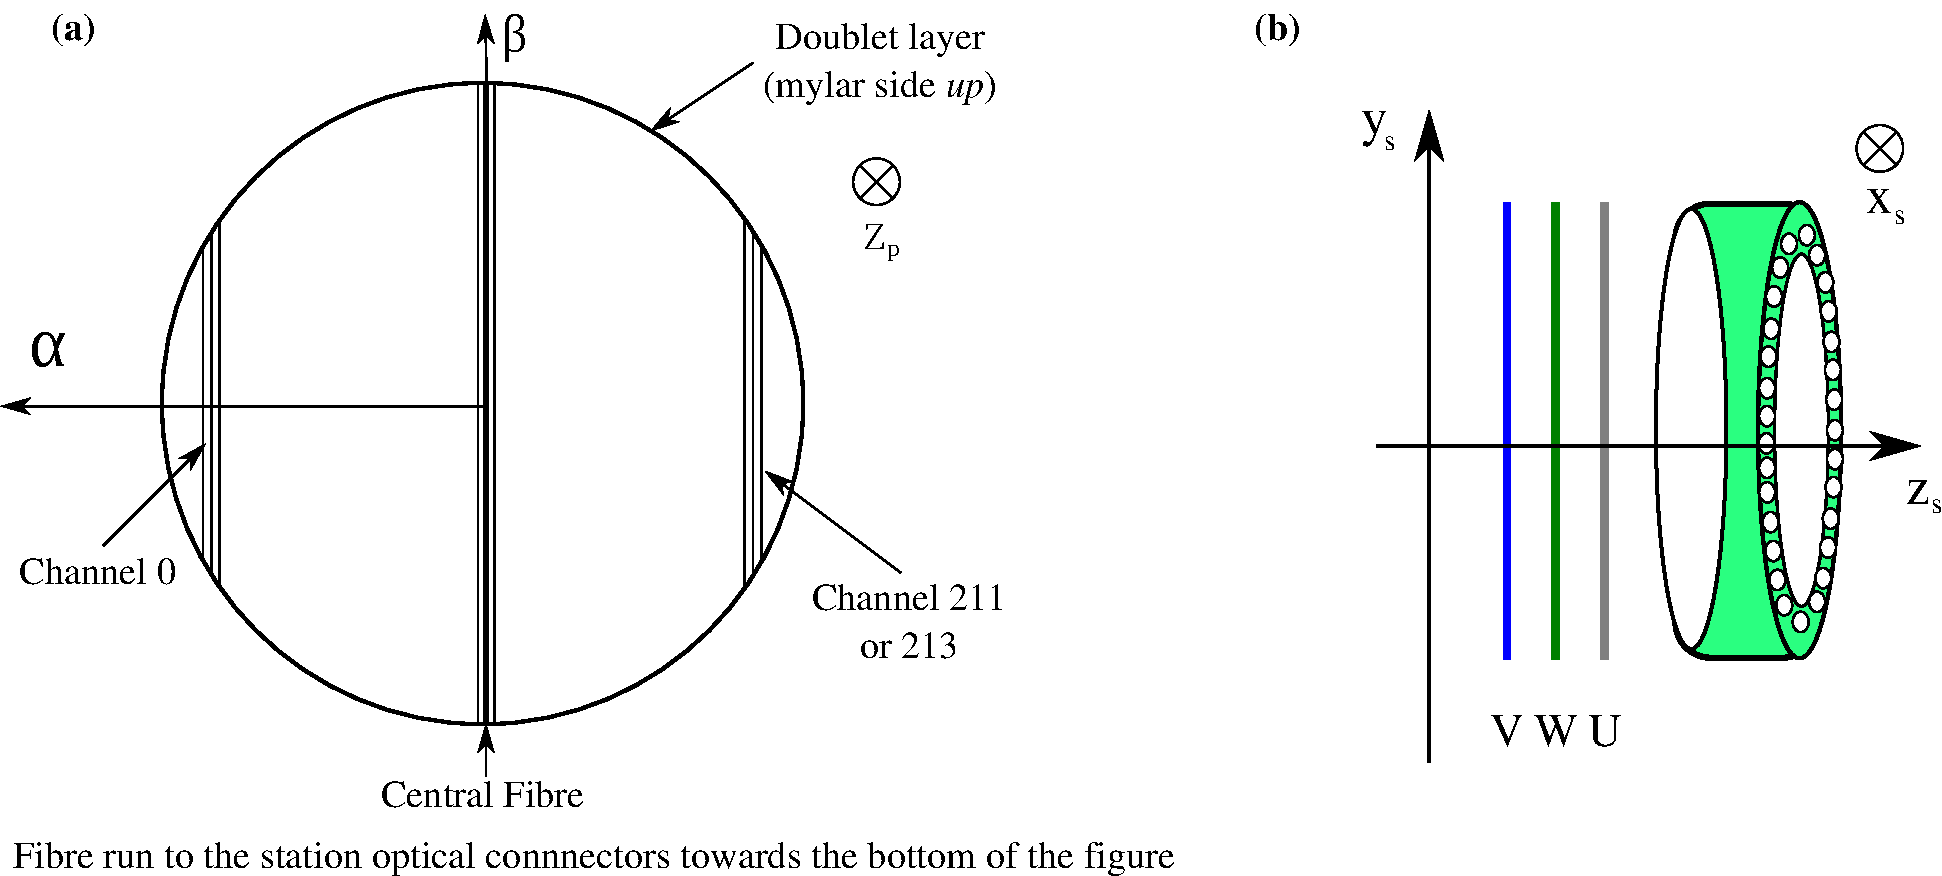
\includegraphics[width=0.9\textwidth]{02-CoordinateSystems/PlaneCoordinatesAndNumbering.pdf}
      \caption{\label{fig:DoubletLayerOrder} (a)~The channel numbering within a plane, and the $(\alpha, \beta, z_p)$ plane coordinate system (a right-handed system).  (b)~The fibre plane ordering with respect to the station body and the $(x_s, y_s, z_s)$ station coordinate frame (a right-handed system).  In TKU the beam approaches from the right, in TKD from the left. Note that $z_s$ is by definition equivalent to $z_p$ of the $V$ plane.}
    \end{center}
  \end{figure}

